\documentclass[11pt,a4paper]{article}
\usepackage{float}
\usepackage[utf8]{inputenc}
\usepackage[left=2cm,right=2cm,text={18cm,24cm},top=2cm]{geometry}
\usepackage[czech]{babel}
\usepackage{graphicx}
\usepackage{verbatim}
\usepackage{fancyvrb}
\usepackage{svg}
\renewcommand{\familydefault}{\sfdefault}

\begin{document}
    \begin{titlepage}
        \begin{center}
            % FIT logo
            
\includegraphics[scale=0.65]{include/fit.pdf} \\

            \LARGE{
                \textbf{
                    Projektová dokumentace} \\
                Překladač jazyka IFJ22} \\
                
            \vspace{2cm}
            
            \Large{
                Tým xstrel03 \\
                Varianta TRP \\
            }
                
            \vspace{2cm}
            
            \normalsize{}
            \today{}

            \vspace{2cm}

            \begin{tabular}{l l l}
                \textbf{Matyáš Strelec} & \textbf{(xstrel03)}   & \quad X\% \\
                Ondřej Seidl            & (xseidl06)            & \quad X\% \\
                Maxmilián Nový          & (xnovym00)            & \quad X\% \\
                Dominik Klon            & (xklond00)            & \quad X\% \\
            \end{tabular}
        \end{center}
    \end{titlepage}

    \tableofcontents

    \pagebreak{}

    \section{Práce v týmu}
    Rozdělení práce mezi členy týmu (uveďte kdo a jak se podílel na jednotlivých
    částech projektu; povinně zdůvodněte odchylky od rovnoměrného rozdělení bodů).
    
    \subsection{Rozdělení práce}

    \subsection*{Matyáš Strelec}
    \begin{itemize}
        \item Lexikální analýza
        \item Syntaktická analýzy
        \item Dokumentace
    \end{itemize}

    \subsection*{Ondřej Seidl}
    \begin{itemize}
        \item Implementace tabulky symbolů
        \item Zpracování výrazů
    \end{itemize}

    \subsection*{Maxmilián Nový}
    \begin{itemize}
        \item Návrh LL-gramatiky
        \item Vestavěné funkce
    \end{itemize}

    \subsection*{Dominik Klon}
    \begin{itemize}
        \item Generování kódu
    \end{itemize}

    \subsection{Odchylky od rozvnoměrného rozdělení}
    

    \pagebreak{}

    \section{Lexikální analýza}

    \subsection{Datové struktury}
    Implementace lexikální analýzy je obsažena v souborech \verb|lexer.c| a \verb|lexer.h|.
    Pro potřeby lexikálního analyzátoru byly vytvořeny datové struktury které pomáhají při
    práci s tokeny a konečným automatem. Výčtový typ \verb|fsm_state_t| obsahuje všechny možné
    stavy konečného automatu dle návrhu, výčtový typ \verb|token_type_t| definuje typy tokenů.
    \\ \\
    Struktura \verb|token_t| obsahuje informace o tokenu, jeho typ, pozici v souboru, délku,
    a jeho předchůdce a následníka ve spojovém seznamu. Struktura \verb|token_list_t| obsahuje
    ukazatele na první, poslední, a aktuální token.

    \subsection{Funkce}

    Všechny funkce jsou ve zdrojových souborech popsané v komentářích, včetně jejich funkcionality, parametrů a návratových hodnot.
    \\ \\
    Funkce lexeru volaná z hlavního programu je funkce \verb|fillTokenList()|, která jako parametr
    dostává ukazatel na strukturu \verb|token_list_t|, kterou naplní seznamem tokenů pomocí volání
    funkce \verb|getNextToken()|. Funkce \verb|getNextToken()| je volána v cyklu, dokud není dosažen token
    typu konec souboru.
    \\ \\
    Funkce \verb|getNextToken()| je implementována pomocí konečného automatu. Dle posloupnosti znaků na vstupu
    určuje typ a vyplňuje data tokenu. V případě, že je na vstupu znak, který nelze podle automatu dále číst,
    je kontrolováno, jestli momentální stav automatu je koncový, pokud ano, token je validní.
    Dále jsou rozpoznána klíčová slova a odstraněny úvozovky z řetězců. Pokud automat není v koncovém stavu,
    ale na vstup přijde znak, který automat nemůže přečíst, funkce vrací chybu 1.
    \\ \\
    Dále soubor obsahuje funkce na práci se seznamem tokenů jako vázaným seznamem a funkce pro ladění.

    \subsection{Diagram konečného automatu}
    Vizte obrázek \ref{fig:fsm}.
    
    \begin{figure}[H]
        \centering
        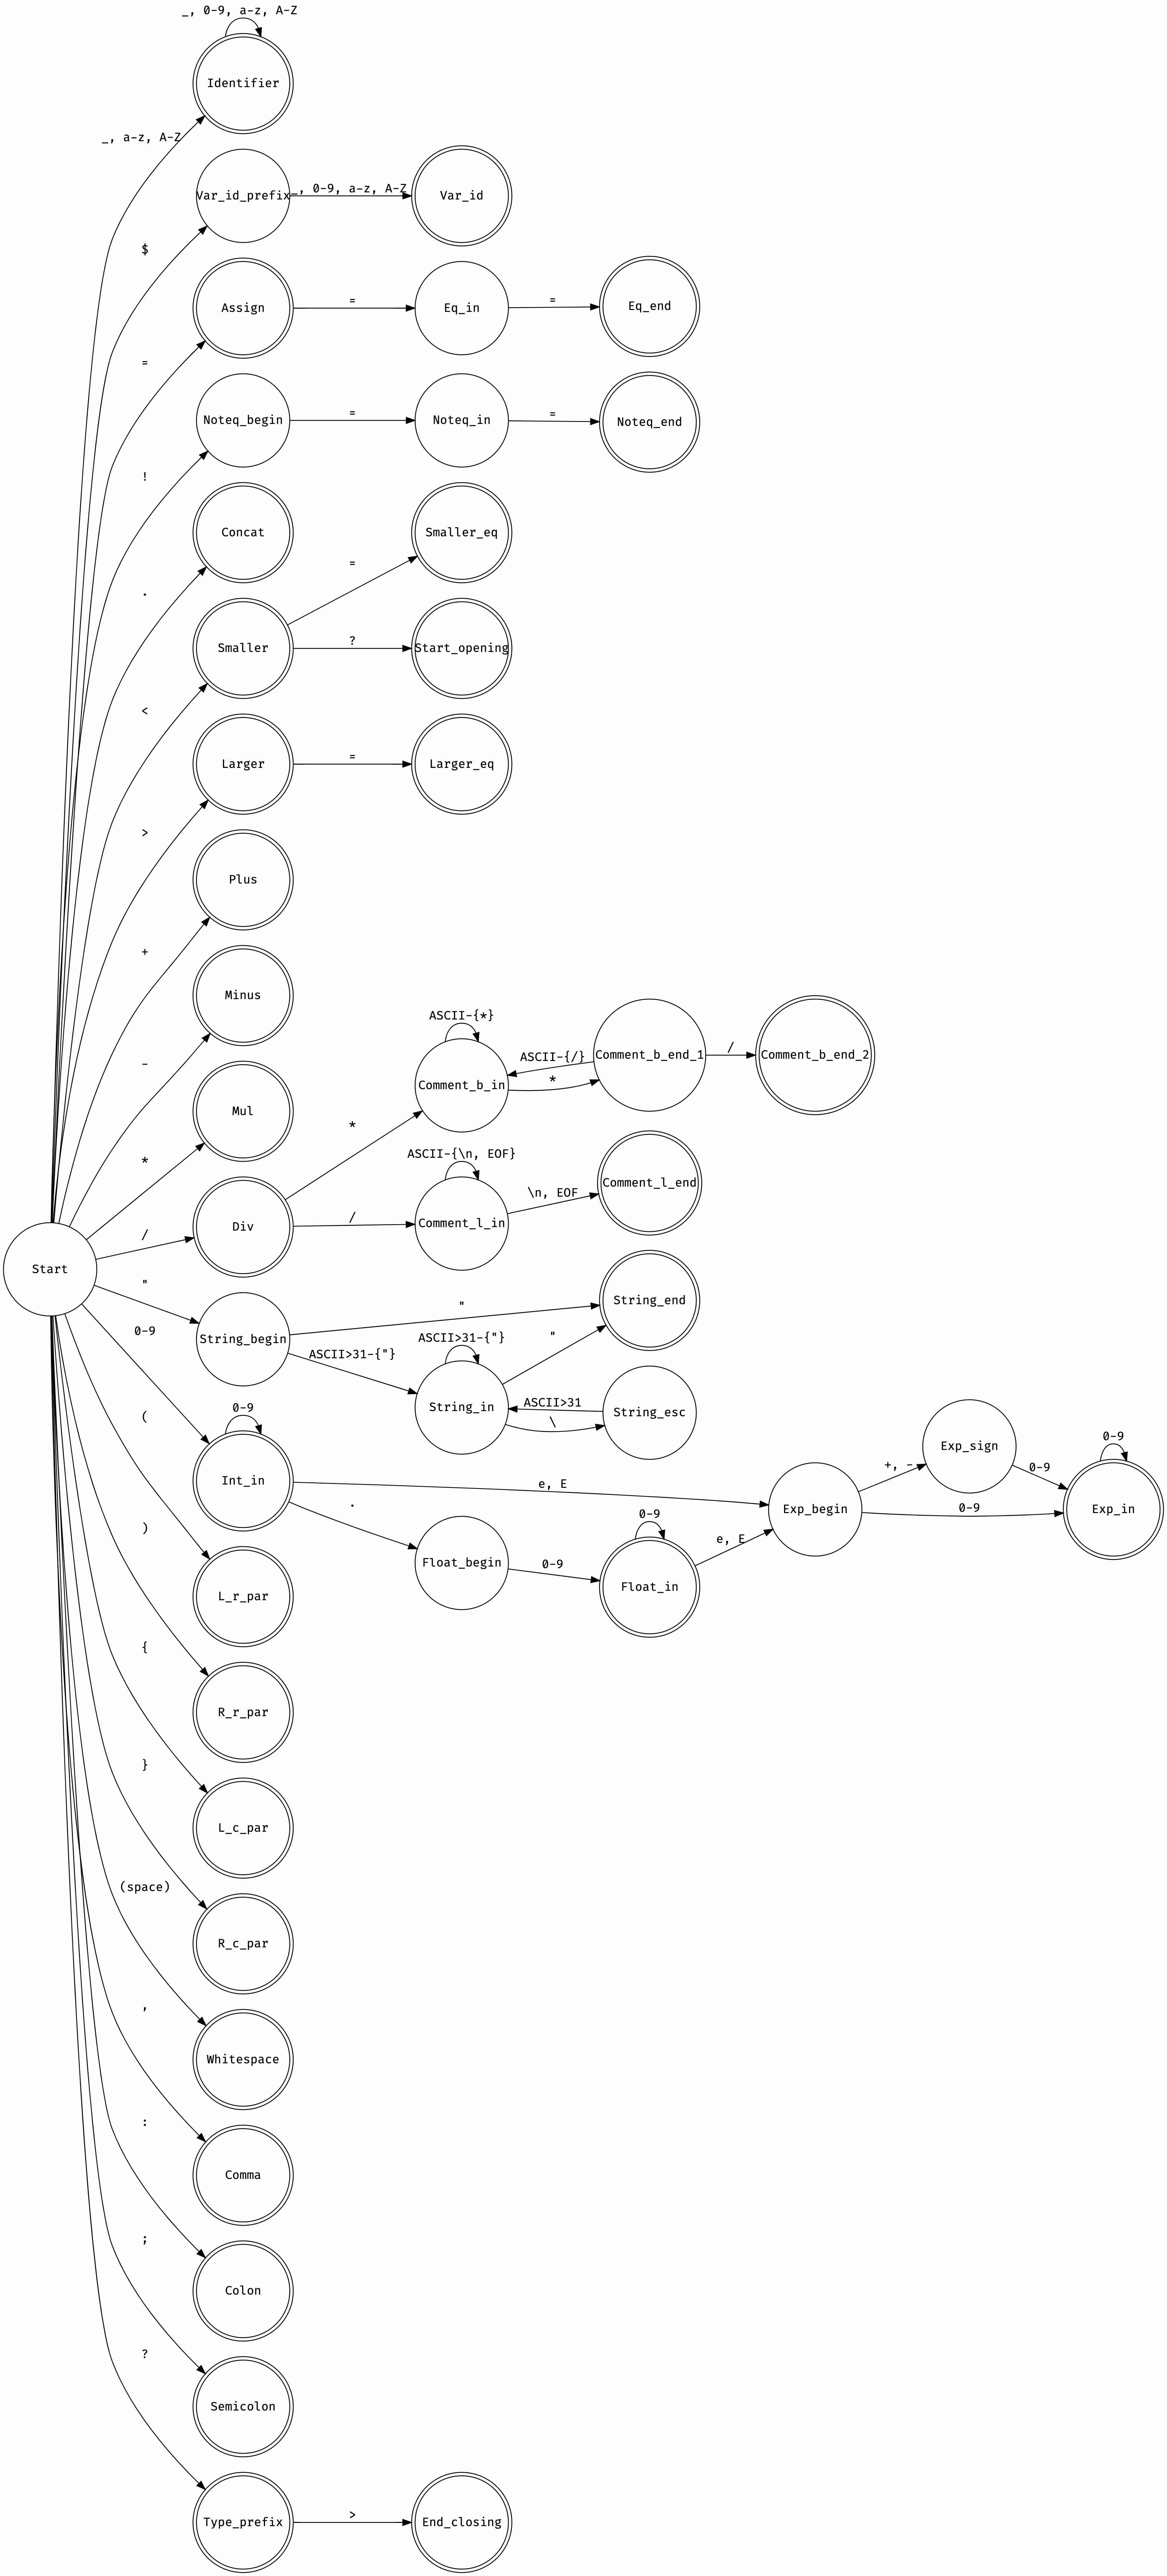
\includegraphics[height=0.97\textheight]{fsm.jpg}
        \caption{Diagram konečného automatu vytvořený nástrojem \texttt{Graphviz}}
        \label{fig:fsm}
    \end{figure}

    \pagebreak{}
    
    \section{Syntaktická analýza}
    
    \subsection{Implementace}

    \subsection{LL-gramatika}
    Pro jazyk IFJ22 byla navržena následující gramatika.
    \begin{Verbatim}
1:  <prog> -> <stat> <prog>
2:  <prog> -> function func-id ( <params> ) : type { <st-list> } <prog>
3:  <prog> -> <eof>

4:  <eof> -> ?> EOF
5:  <eof> -> EOF

6: <params-cont> -> , type $id <params-cont>
7: <params-cont> -> eps

8: <params> -> type $id <params-cont>
9: <params> -> eps

10: <args-cont> -> , <term> <args-cont>
11: <args-cont> -> 

12: <args> -> <term> <args-cont>
13: <args> -> eps

14: <stat> -> $id = <assign> ;
15: <stat> -> while ( <expr> ) { <st-list> }
16: <stat> -> if ( <expr> ) { <st-list> } else { <st-list> }
17: <stat> -> return <expr> ;
18: <stat> -> <expr> ;
19: <stat> -> func-id ( <args> ) ;

20: <st-list> -> <stat> <st-list>
21: <st-list> -> eps

22: <assign> -> <expr>
23: <assign> -> func-id ( <args> )

24: <term> -> $id
25: <term> -> val
    \end{Verbatim}
    \subsection*{Poznámky}
        \texttt{\$id} - identifikátor proměnné\\
        \texttt{func-id} - identifikátor funkce\\
        \texttt{val} - číselný nebo řetězcový literál \\
        \texttt{type} - datový typ (\texttt{int}, \texttt{double}, \texttt{string}) \\
        \texttt{func-id} - identifikátor funkce \\
        \texttt{eps} - $\varepsilon$ \\

    \subsection{LL-tabulka}

    \subsection{Precedenční tabulka}


    \section{Sémantická analýza}


    \section{Tabulka symbolů}


    \section{Generování kódu}


    \section{Zpracování výrazů}


    \section{Chybové hlášení}


    \section{Hlavní program}

\end{document}
